\subsection{Rings}
\label{subsec:rings}

We have seen in the proof of the five color theorem that a vertex surrounded by five or less neighbors can always be colored using one of five colors, even if all of its neighbors initially use all five colors. If we have only four colors available, we will find that it is no longer guaranteed that we can free a color. This is what Alfred Kempe tried to do when he gave the first false proof of the four color theorem.

If we look at the key idea, we see that if one half of a graph is isolated from another half by a group of boundary vertices, we can color this isolated part regardless of the colors on the boundary. Naturally, the fundamental shape that seperates a graph in two halves is a \textit{ring} (or a line if it is not cyclic).

\begin{definition}
    A \emph{ring} of $n$ vertices $R_n$ in a planar graph $G$ is an induced cycle of $G$.
\end{definition}

An example of what is a ring and what is not can be seen in Figure \ref{fig:ring}.

\begin{figure}[!ht]
    \centering
    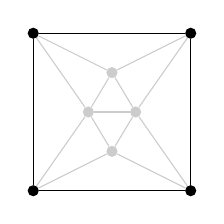
\begin{tikzpicture}
        \node[circle, fill, scale=0.015cm] (l1) at (-1, -1) { };
            \node[circle, fill, scale=0.015cm] (l2) at (-1, 1) { };
            \node[circle, fill, scale=0.015cm] (l3) at (1, 1) {};
            \node[circle, fill, scale=0.015cm] (l4) at (1, -1) {};
            \node[circle, fill, scale=0.015cm, opacity=0.2] (m1) at (0, 0.5) {};
            \node[circle, fill, scale=0.015cm, opacity=0.2] (m2) at (-0.3, 0) {};
            \node[circle, fill, scale=0.015cm, opacity=0.2] (m3) at (0.3, 0) {};
            \node[circle, fill, scale=0.015cm, opacity=0.2] (m4) at (0, -0.5) {};

            \draw (l1) -- (l2) -- (l3) -- (l4) -- (l1);
            \draw[opacity=0.2] (m1) -- (m2) -- (m4) -- (m3) -- (m1);
            \draw[opacity=0.2] (m2) -- (m3);
            \draw[opacity=0.2] (m1) -- (l2);
            \draw[opacity=0.2] (m1) -- (l3);
            \draw[opacity=0.2] (m2) -- (l1);
            \draw[opacity=0.2] (m2) -- (l2);
            \draw[opacity=0.2] (m3) -- (l3);
            \draw[opacity=0.2] (m3) -- (l4);
            \draw[opacity=0.2] (m4) -- (l1);
            \draw[opacity=0.2] (m4) -- (l4);
    \end{tikzpicture}
    \hspace{1cm}
    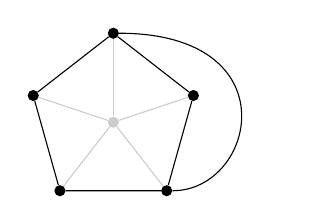
\begin{tikzpicture}[scale=1.13]
        \node[circle, fill, scale=0.015cm, opacity=0.2] (c) at (0, 0) {};


        \node[circle, fill, scale=0.015cm] (l1) at (0, 1) { };
        \node[circle, fill, scale=0.015cm] (l2) at (0.9, 0.30) { };
        \node[circle, fill, scale=0.015cm] (l3) at (0.6, -0.77) {};
        \node[circle, fill, scale=0.015cm] (l4) at (-0.6, -0.77) {};
        \node[circle, fill, scale=0.015cm] (l5) at (-0.9, 0.30) {};

        \draw[opacity=0.2] (c) -- (l1);
        \draw[opacity=0.2] (c) -- (l2);
        \draw[opacity=0.2] (c) -- (l3);
        \draw[opacity=0.2] (c) -- (l4);
        \draw[opacity=0.2] (c) -- (l5);
        \draw (l1) -- (l2) -- (l3) -- (l4) -- (l5) -- (l1);
        \draw (l1) .. controls +(2,0) and +(1,0) .. (l3);
    \end{tikzpicture}
    \caption{In bold, an example of the ring $R_4$ surrounding a graph on four vertices (left) and an example of an invalid ring $R_5$. No extra edges are allowed between ring vertices, since otherwise the ring is not an induced cycle of $G$. }
    \label{fig:ring}
\end{figure}

We will frequently need all the possible colorings for a ring $R$ contained in a certain planar graph $G$. Let us give a name to the set of such colorings.

\begin{definition}
    The set of all 4-colorings of a ring $R$ in a planar graph $G$ is given by $\Phi(R \subset G)$ or $\Phi(G)$ if $R$ is clear from the context. We let $\Phi(n) = \Phi(R_n)$, the set of all possible ring colorings of $R_n$.
\end{definition}

The first thing we might do with rings is see if they themselves are reducible. In fact, we will find a common result from literature.

\begin{theorem}
    \label{thm:ringsarered}
    The ring $R_n$ with $n\geq 4$ is reducible in every planar graph $G$.
\end{theorem}

\begin{proof}
Let $R_n$ be strongly-contained in $G$. Since the interior of $R_n$ is empty and $n\geq4$, we may contract any two non-neighboring ring vertices $u$ and $v$ to a new vertex $y$. As a result, we obtain the graph $G'$ on one less vertex. 

Given a 4-coloring of $G'$. Because $R_n$ is a ring, there will be no edges between the ring vertices $u$ and $v$. Therefore, we may give $u$ and $v$ the same color as $y$ without issue. Let the other vertices of $G$ be given the same color as their $G'$ counterparts. Then we have obtained a 4-coloring of $G$.

\end{proof}

\begin{figure}[!ht]
    \centering
    \begin{tikzpicture}[scale=0.7]
        \node (l1) at (-1, -1) { $a$ };
        \node (l2) at (-1, 1) { $b$ };
        \node (l3) at (1, 1) { $c$ };
        \node (l4) at (1, -1) { $b$ };

        \draw (l1) -- (l2) -- (l3) -- (l4) -- (l1);
        \node (impl) at (2.3, 0) { $\Longleftrightarrow$ };
        \draw[dotted, thick] (l2) -- (l4);
    \end{tikzpicture}
    \begin{tikzpicture}[scale=0.7]
        \node (l1) at (-1, -1) { $a$ };
        \node[opacity=0.2] (l2) at (-1, 1) { $b$ };
        \node (l3) at (1, 1) { $c$ };
        \node[opacity=0.2] (l4) at (1, -1) { $b$ };
        \node (c) at (0, 0) { $b$ };

        \draw (l1) -- (c) -- (l3);
        \draw[dotted, thick, opacity=0.2] (l2) -- (c) -- (l4);
    \end{tikzpicture}
    \caption{The ring $R_4$ being contracted to a smaller graph $G'$. The coloring of $G'$ can be reversed to a coloring of $G$.}
\end{figure}

In the next section we will be treating the reducibility of configurations with a ring as their boundary. It might not be a surprise then that the reducibility of plain rings is a key ingredient in the reducibility of these configurations, too. In Section \ref{sec:creduce} we will see that this form of reducibility with contractions is actually C-reducibility. Therefore, in the context of Theorem \ref{funda1}, plain rings can be considered as C-reducible configurations. 